\documentclass[12pt]{report}
\input{../bayesuvius.sty}
\begin{document}

We will use the units 
used in High Energy
Physics in which $\hbar$ (Plank's constant divided by $2\pi$) and $c$ (speed of light) are set to 1 
temporarily, and then restored when one needs actual values in MKS units. In such units,
everything has dimensions of $L^D$, where $L$
stands for length, and $D$ is some rational number. The dimensions of length and time are $L$ and those of energy, mass and
momentum are $L^{-1}$.

Assume Euclidean metric.

Let

$ \phi(x)$ =  field at point $x\in \RR^d$

$m$ = mass of particle

$\lambda$ = coupling constant


Bare Lagrangian density
in Euclidean metric for
$\phi^4$ theory in $d$ dimensions is
(bare quantities have zero subscript)


\beq
\call_0 =
\frac12 \sum_{j=1}^d(\partial_{x_j} \phi_0)^2
+
\frac12 m_0^2 \phi_0^2
+
\frac{\lambda_0}{4!}\phi_0^4
\eeq


\beq
\engdim{\int d^d x \call_0}
=L^0
\eeq


Let
\beq
\epsilon = 4-d
\eeq
Then define


\beq
\phi_0 = Z_\phi^{1/2}\phi(\mu)
\eeq

\beq
m_0^2 = Z_m m^2(\mu)
\eeq

\beq
\lambda_0 = \mu^\epsilon Z_\lambda \lambda(\mu)
\label{eq-lam-bare-mu-eps}
\eeq

\begin{claim}
\beq
\engdim{\phi_0}=\engdim{\phi}= L^{\frac{2-d}{2}},\quad
\engdim{m^2_0}=\engdim{m^2}=L^{-2}
\eeq
\end{claim}
\proof
\beq
L^0=\engdim{(d^dx) (\partial_{x_i} \phi)^2}
=
L^d L^{-2} \engdim{\phi}^2
\eeq
\qed

\begin{claim}
The factor $\mu^\epsilon$ 
in Eq.(\ref{eq-lam-bare-mu-eps}) 
is introduced to make the coupling constant $\lam$
 dimensionless and the bare
coupling constant dimensionful.

\beq
\engdim{\lam}=L^0, \quad \engdim{\lam_0}= L^{-\eps}
\eeq
\end{claim}
\proof

Assume $\phi^n$
interaction and $\engdim{\lam_0}=L^{-p}$

\beq
L^0=
\engdim{(d^dx)\lam_0 \phi^n_0}=
L^d L^{-p}L^{\frac{n(2-d)}{2}}
\eeq

\beq
0=d-p+ \frac{n(2-d)}{2}
\eeq
\beq
p= d + n -\frac{nd}{2}
\eeq
If $n=4$,

\beq
p=4-d
\eeq
If we now set
$\eps= 4-d$,
we get
\beq
p=\eps
\eeq

In the $\phi^3$
theory in 6 dimensions considered
in Srednicki's book Ref.-------------------%\cite{Sr},
one gets, with $n=3$, that

\beq
p= 3-\frac{d}{2}= \frac{6-d}{2}\eeq
If we now set $\eps =6-d$, we get
\beq
p= \frac{\epsilon}{2}
\eeq
\qed



%\beqa
%\call_0&=&
%Z_\phi\left[
%\frac12
%(\partial_\mu \phi)^2
%+
%Z_m m^2 \phi^2
%+
%\mu^\eps Z_\lam Z_\phi
%\frac{\lambda}{4!}\phi^4
%\right]
%\\
%&=&
%\call + \Delta \call
%\eeqa
%Counterterms $\Delta\call$
%
%\beq
%\Delta \call=
%=\left\{
%\begin{array}{l}
%(Z_\phi-1)
%\frac12
%(\partial_\mu \phi)^2
%\\
%+
%(Z_mZ_\phi -1)m^2 \phi^2
%\\
%+
%(\mu^\eps Z_\lam Z_\phi^2-1)
%\frac{\lambda}{4!}\phi^4
%\end{array}
%\right.
%\eeq

\begin{subequations}
\label{eqs-micro-no-change}
\beq
\frac{d}{d\mu} \phi_0 =0
\eeq
\beq
\frac{d}{d\mu} m_0^2 =0
\eeq
\beq
\frac{d}{d\mu} \lambda_0 =0
\eeq
\end{subequations}
The physical reason 
for Eqs.(\ref{eqs-micro-no-change})
is, in the words of
 Ken Wilson: \qt{The microscopic theory is fixed while the effective couplings change as we change the scale.}


The bare theory does not depend on the arbitrary renormalization scale
$\mu$.
Because the bare parameters are $\mu$-independent, the renormalized ones must \qt{run}.

Define

field anomlous dimension
\beq
\gamma_\phi =
-\;\frac{d \ln \phi}{d\ln \mu}
\eeq

 

 mass anomalous dimension

\beq
\gamma_m =
-\;\frac{d \ln m^2}{d\ln \mu}
\eeq

beta function

\beq
\beta =
 \frac{d\lambda}{d\ln \mu}
\eeq


\beqa
\Gamma^{(4)}&=&
Z_\phi^2\left[
\bcen
\xymatrix{
\ar@{-}[dr]
&
&
\\
& \ar@{-}[ur]\ar@{-}[dr]\lam_0
&
\\
\ar@{-}[ur]
&
&
}
\ecen
+
3
\bcen
\xymatrix{
\ar@{-}[dr]
&
&
&
\\
&\ar@{-}@/_1pc/[r]\ar@{-}@/^1pc/[r]
\lam_0
& \ar@{-}[ur]\ar@{-}[dr]\lam_0
&
\\
\ar@{-}[ur]
&
&
&
}
\ecen
+\calo(\lam_0^3)
\right]
\\
&=&
Z_\phi^2\left[
\lam_0+  \lam_0^2 3\cali
\right]
\eeqa

3 equal one-loop integrals $\cali$, one for each channel (s, t, u)

\beq
\cali = \int \frac{d^d k}{(2\pi)^d}
\frac{1}{(k^2 + m^2)((k+p)^2 + m^2)}
\eeq
\begin{mdframed}[hidealllines=true,backgroundcolor=blue!10]
\begin{claim}
\beq
\cali=
\frac{2}{(4\pi)^2}
\left(
\frac{1}{\eps}
-\frac{1}{2}\int_0^1 dx\;\ln\left(\frac{\Delta}{4\pi e^{-\gamma_E}}\right)
\right)
+\calo(\eps)
\eeq

\beq
\Delta = m^2 + x(1-x)p^2
\eeq
\end{claim}
\proof

Use Feynman parameters:
\beq
\frac{1}{AB} = \int_0^1 dx \frac{1}{[xA + (1-x)B]^2}
\eeq

So:
\beq
\cali = \int_0^1 dx \int \frac{d^d k}{(2\pi)^d}
\frac{1}{\left[(k + xp)^2 + \Delta\right]^2}
\eeq



Shift $k \to k - xp$:

\beq
\cali = \int_0^1 dx \int \frac{d^d k}{(2\pi)^d}
\frac{1}{(k^2 + \Delta)^2}
\eeq

Dimensional regularization integral
Standard formula:

\beq
\int \frac{d^d k}{(2\pi)^d}
\frac{1}{(k^2 + \Delta)^2}
=
\frac{1}{(4\pi)^{d/2}}
\Gamma\left(2-\frac{d}{2}\right)
\Delta^{\frac{d}{2} - 2}
\eeq

Set $d = 4 - \epsilon$:


\beq
\cali=
\frac{1}{(4\pi)^{2-\eps/2}}
\Gamma\left(\frac{\eps}{2}\right)
\int_0^1 dx\;
\Delta^{-\frac{\eps}{2}}
\eeq

Expand everything

\beq
\Gamma\left(\frac{\eps}{2}\right)
\approx
\frac{2}{\eps}-\gamma_E  + \calo(\eps)
\eeq
$\gamma_E \approx 0.58$ Euler constant

\beq
\left(\frac{\Delta}{4\pi}\right)^{-\frac{\eps}{2}}
= 1 -\frac{\eps}{2}\ln\left(\frac{\Delta}{4\pi}\right)+\calo(\eps^2)
\eeq
Multiply pieces

\beqa
\cali&=&
\frac{1}{(4\pi)^2}
\left(
\frac{2}{\eps} -\gamma_E 
-\int_0^1 dx\;\ln\left(\frac{\Delta}{4\pi}\right)
\right)
\\
&=&
\frac{2}{(4\pi)^2}
\left(
\frac{1}{\eps}
-\frac{1}{2}\int_0^1 dx\;\ln\left(\frac{\Delta}{4\pi e^{-\gamma_E}}\right)
\right)
\eeqa

\qed
\end{mdframed}
\begin{claim}(no wavefunction renormalization at 1-loop)
\beq
Z_\phi = 1 + O(\lambda^2)\eeq
\end{claim}
\proof
\qed

\begin{claim}
\beq
Z_\lam = 1 + \lam a\left(
\frac{1}{\eps}-b\right) +\calo(\lam^2)
\eeq
where
\beq
a= \frac{3}{(4\pi)^2}\approx 0.0190,
\quad 1/a\approx 52.6
\eeq

\beq
\left\{
\begin{array}{ll}
b=0 &
\text{if Minimal Subtraction  (MS)}
\\
b = \gamma_E - \ln(4\pi) &
 \text{if Modified Minimal Subtraction  (MMS)}
\end{array}
\right.
\eeq

\end{claim}
\proof
\qed


\begin{claim}
If
\beq
\left\{
\begin{array}{l}
\lam_0 =
\mu^\eps Z_\lam\tilde{\lam}
\\
\tilde{\lam}=
\lam[1 + ab\lam + \calo(\lam^2)]
\end{array}
\right.
\eeq
or

\beq
\left\{
\begin{array}{l}
\lam_0 =
\tilde{\mu}^\eps Z_\lam\lam
\\
\tilde{\mu}=\mu e^{b}
\end{array}
\right.
\eeq
then $\lam_0$ is independent of $b$.
It equals

\beq 
\lam_0=\mu^\eps \lam
\left[1+
\frac{\lam a}{\eps}
 + \calo(\lam^2)
\right]
\eeq
\end{claim}
\proof

\beqa
\lam_0 
&=&
\mu^\eps \lam
\left[1+
\lam a\left(
\frac{1}{\eps}-b\right)
+ ab\lam + \calo(\lam^2)
\right]
\\
&=&
\mu^\eps \lam
\left[1+
\frac{\lam a}{\eps}
 + \calo(\lam^2)
\right]
\eeqa
\beq
\tilde{\mu}^\eps=
\mu^\eps\left(1 +\eps b
+\calo(\eps^2)\right)
\eeq

\beqa
\lam_0 &=& 
\mu^\eps\left(1 +\eps b
+\calo(\eps^2)\right)
\left[
 1 + \lam a\left(
\frac{1}{\eps}-b\right) +\calo(\lam^2)
\right]\lam
\\
&=&
\mu^\eps
\left(
 1 + \lam a\left(
\frac{1}{\eps}-b\right)
+\lam ab
\right)\lam
\\
&=&
\mu^\eps
\left(
 1 +
\frac{\lam a}{\eps}
\right)\lam
\eeqa

\qed


\begin{claim} 

\beq
\boxed{\beta(\lam)=
-\epsilon \lambda
+a\lam^2}
\eeq


\end{claim}
\proof



\beq
\lam_0=
\mu^\eps \lam
\left[1+\frac{\lam a}{\eps} +\calo(\lam^2)
\right]
\eeq

\beqa
0&=&\mu\frac{d\lam_0}{d\mu}
\\
&=&
\mu\frac{d}{d\mu}
\left(\mu^\eps
\left[\lam+\frac{\lam^2 a}{\eps}
+\calo(\lam^3) 
\right]\right)
\\
&=&
\eps\mu^\eps
\left[\lam+\frac{\lam^2 a}{\eps}
\right]
+
\mu^\eps \beta(\lam)
\left[1+\frac{2\lam a}{\eps}
\right]
+
\calo(\lam^3)
\eeqa

\beqa
\beta(\lam)
&=&
-\eps\lam
\frac{1+\frac{\lam a}{\eps}}
{1+\frac{2\lam a}{\eps}} +\calo(\lam^3)
\\
&=&
-\eps\lam\left(
1-\frac{\lam a}{\eps} 
\right)+\calo(\lam^3)
\\
&=& -\eps\lam +a \lam^2
\eeqa
\qed


Set
\beq
\beta(\lambda_*) =0
\eeq

This gives the {\bf Wilson–Fisher fixed point}

\beq
\lambda_* =
\frac{\epsilon}{a}
\approx 52.6 \eps
\eeq

For $d=4$, 
$
\epsilon=0
$
so the fixed point is Gaussian.
For $d<4$ a non-trivial fixed point appears.
This fixed point describes the {\bf Ising universality class}.

\section{$\phi^4$ to Ising}

The critical point of the $\phi^4$ theory and that of the Ising model
are
in the same universality class.
Near the critical point

\beq
m^2 \propto \frac{T-T_c}{T_c} = t
\eeq
so the mass parameter corresponds to temperature deviation.

Thus the RG equation

\beq
\frac{d\ln m^2}{d\ln\mu}=
-\gamma_m
\eeq
is exactly the field-theory version of

\beq
\frac{d\ln t}{d\ln b}=
y_t
\eeq
where

\beq
y_t = -\gamma_m=\frac{1}{\nu}
\eeq





\section{Coupling behavior near fixed points}



\beq
\int_{\lam_0}^\lam\frac{d\lam}{\beta(\lam)}=\int_{\mu_0}^\mu d\ln(\mu)
\eeq

\beqa
\beta(\lam) &=& -\eps\lam + a\lam^2 +\calo(\lam^3)
\\
&=&
a\lam(\lam-\lam^*)
\quad \text{with } \lam^*=\frac{\eps}{a}
\eeqa

\beq
\beta(\lam)= a(\lam-\lam^*_1)(\lam-\lam^*_2)\ldots(\lam-\lam^*_n)
\eeq

\beq
\beta(\lam)\approx (\lam-\lam^*_1)
\underbrace{a(\lam^*_1-\lam^*_2)\ldots(\lam^*_1-\lam^*_n)}_R
\eeq

\beq
\ln\frac{|\lam-\lam^*|}
{|\lam_0-\lam^*|}
=R
\ln\frac{\mu}{\mu_0}
\eeq


%
%\beq
%\frac{d\lam}{d\ln\mu}=a\lam^n
%\eeq
%
%For $n=1$,
%
%\beq
%\frac{1}{a}\ln\left(\frac{\lam(\mu)}{\lam(\mu_0)}\right)=
%\ln\left(\frac{\mu}{\mu_0}\right)
%\eeq
%Define
%\beq
%K(\lam, \mu)= \frac{1}{a}\ln\left(\frac{1}{\lam(\mu)}\right) +\ln\mu
%\eeq
%
%For $n>1$
%\beq
%\frac{1}{\lam^{n-1}(\mu)}
%-
%\frac{1}{\lam^{n-1}(\mu_0)}
%=
%-(n-1)a\ln\left(\frac{\mu}{\mu_0}\right)
%\eeq
%Define
%\beq
%K(\mu, \lam)=\frac{1}{(n-1)a \lam^{n-1}(\mu)} +\ln \mu
%\eeq
%
%\beq
%K(\lam,\mu)=K(\lam_0, \mu_0)
%\eeq
%
%\begin{figure}[h!]
%\centering
%\includegraphics[width=5.9in]
%{running-coupling.png}
%\caption{Running Coupling constant $\lam(\mu)$
%for $\beta=a\lam^n$ for
%cases $n=1$ and $n>1$.}
%\label{fig-running-coupling}
%\end{figure}

\section{Beta function from a potential}

Newton's equation says 
\beq
m\ddot{x}= F
\eeq
where $m=$mass, $x=$ position, and $F=$ force. But
you could  have, once the acceleration dies down,
an equilibrium between a drag force and a propulsion force. Let

$\gamma \dot{x}=$ drag,  a velocity dependent force with $\gamma>0$

$F=-\partial_x V=$ propulsion, a conservative force with potential function $V$

Then, at equilibrium,

\beq \gamma\dot{x}=F = -\partial_x V
\label{eq-phi-four-drag-prop}
\eeq

Note that

\beq
\gamma\partial_x\dot{x}=F = -\partial_x^2 V
\eeq


As shown in Fig.\ref{fig-V-derivatives-phi-four},
$V$ has positive second derivative
(hold water convexity)
on both sides of a {\bf stable, attractive fixed  point (attractor, sink)},
and it has negative second derivative
(drop water convexity)
on both sides of an {\bf unstable, repulsive fixed point (repeller, source)}. Hence, we can think of
$V$ as a potential in which a ball rolls towards an attractor
and away from a repeller.



\begin{figure}[h!]
\centering
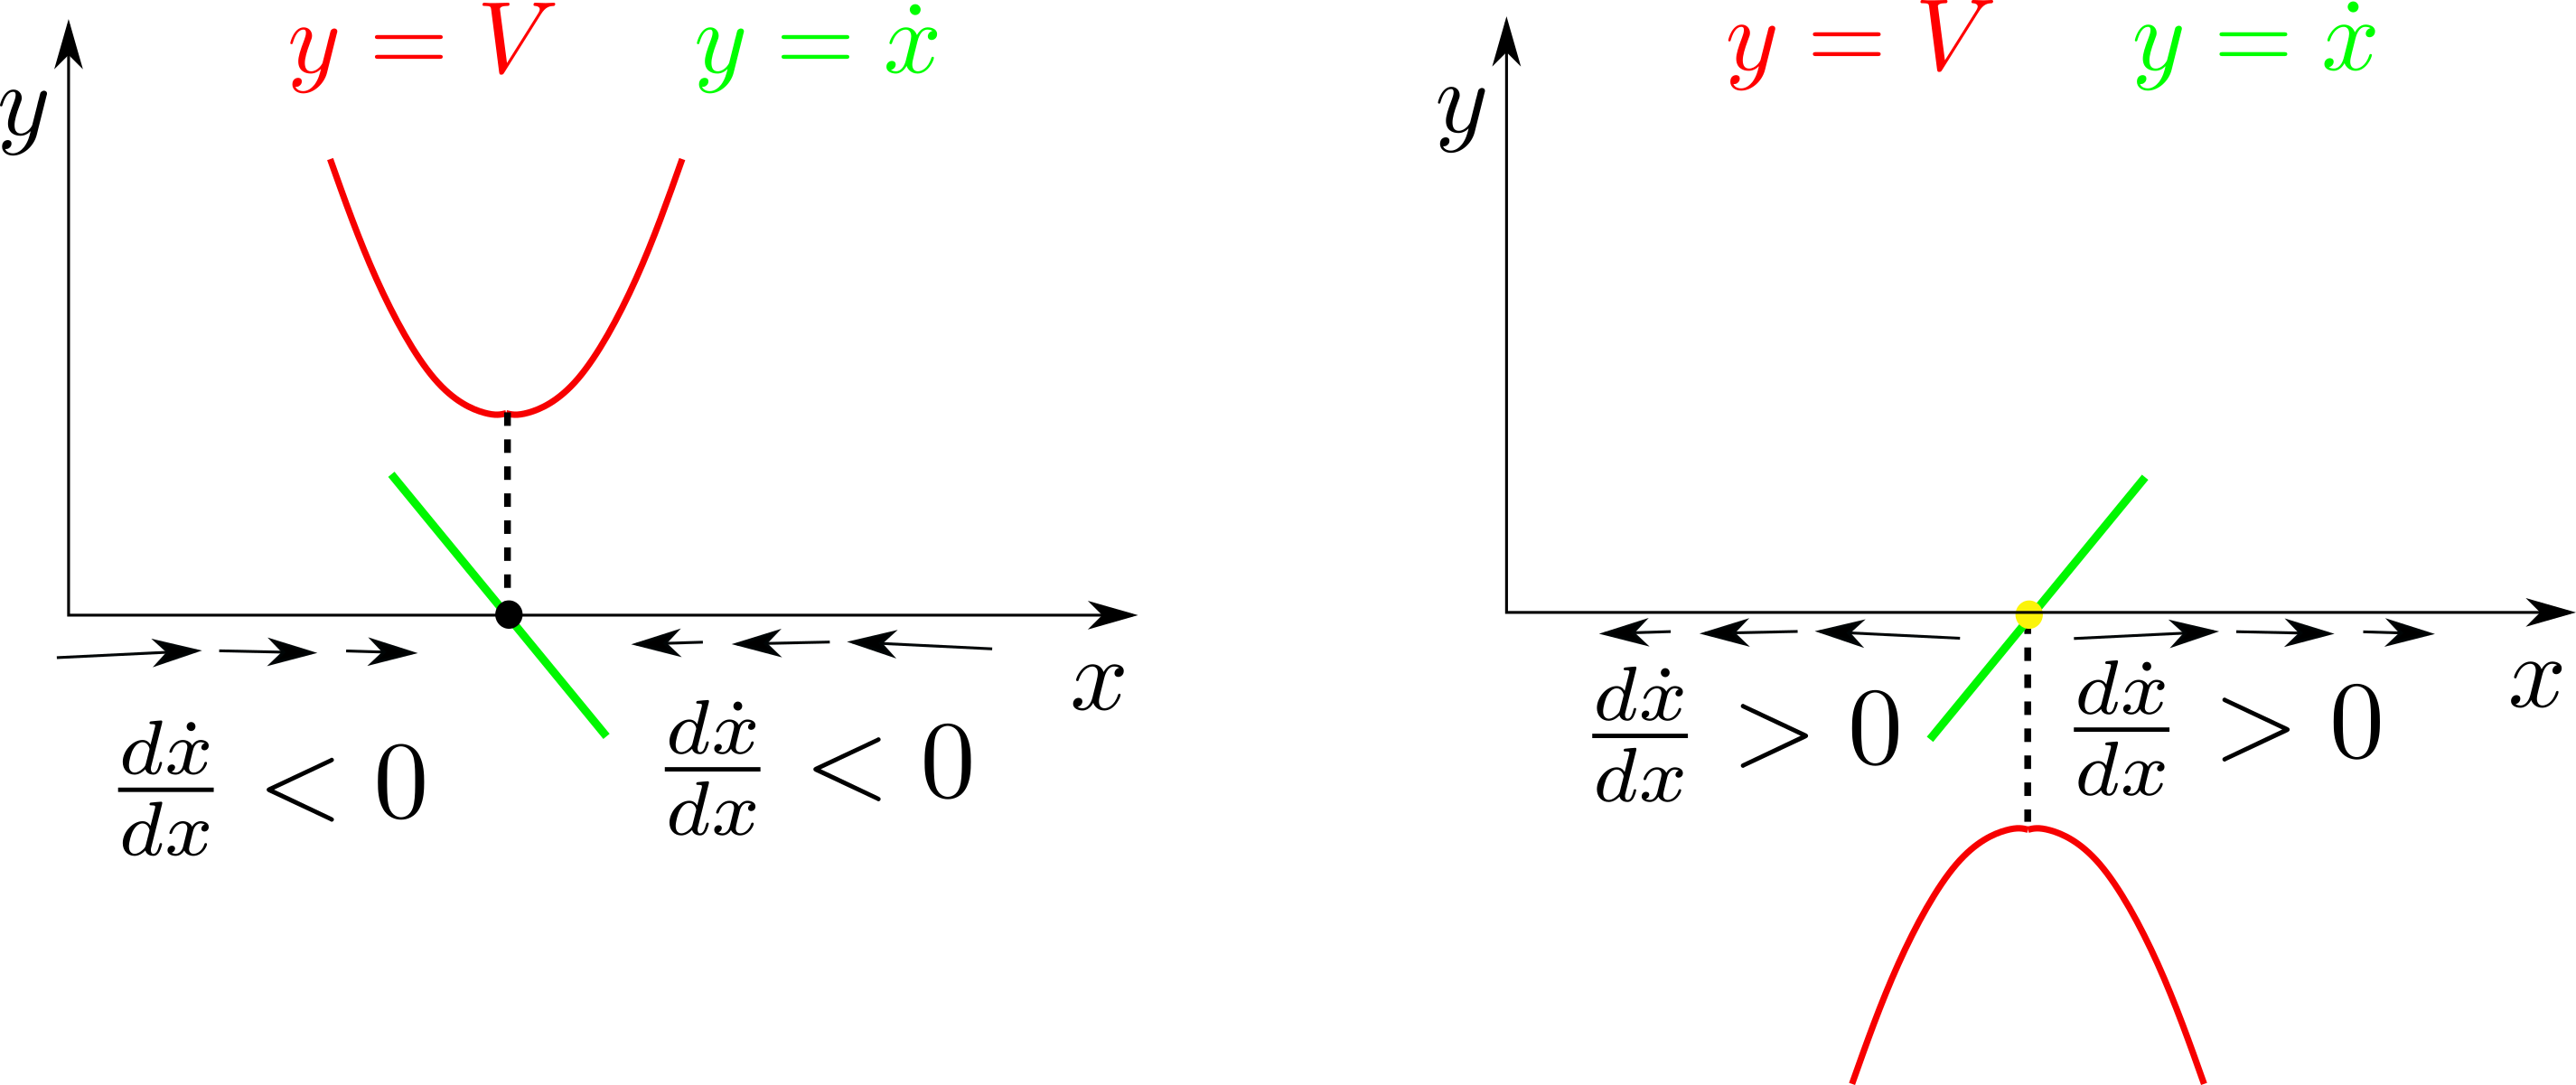
\includegraphics[width=4in]
{../dynamical-sys/V-derivatives.png}
\caption{Illustration of
$\frac{d\dot{x}}{dx}=-\partial^2_xV$. Arrows
in vector field are 
proportional to $\dot{x}$. }
\label{fig-V-derivatives-phi-four}
\end{figure} 

Now 
set
position =$x\rarrow \lam$, time=$t\rarrow \ln \mu$,
and $\gamma=1$
in Eq.(\ref{eq-phi-four-drag-prop})

\beq
\frac{d \lam}{dt}= \beta(\lam) = -\partial_\lam V
\eeq

\beq
V(\lam)-V(\lam_0)
=
-\int_{\lam_0}^\lam
d\lam\; \beta(\lam)
\eeq

\beq
\beta(\lam)= -\eps \lam + a\lam^2
\implies V(\lam)= \frac{\eps}{2}\lam^2-
\frac{a}{3}\lam^3 + \text{constant}
\eeq

Minimum at $\lam=0$ and maximum at

\beq
0=\partial_\lam V(\lam^*)=-\beta(\lam^*)
\implies \quad
\lam^*=\frac{\eps}{a}
\eeq
Wilson-Fisher fixed point (Curie point)


\section{tempo}

 7. Insert $\mu^\epsilon$

Each vertex contributes $\mu^\epsilon$, so diagram has $\mu^{2\epsilon}$.

Expand:
$$
\mu^{2\epsilon}
= 1 + 2\epsilon \ln \mu + O(\epsilon^2)
$$

Multiply with $2/\epsilon$:

$$
\mu^{2\epsilon} \cdot \frac{2}{\epsilon}
=\frac{2}{\epsilon} + 4\ln \mu
$$

So the full divergent + log structure becomes:

$$
\frac{2}{\epsilon}
\gamma
- \ln 4\pi
- 2\ln \mu^2
\ln \Delta
  $$

Combine logs:
$$
\ln \left(\frac{\mu^2}{\Delta}\right)
$$

---

 8. Final 1-loop correction

Including combinatorics (3 channels):

$$
\mathcal{M}^{(1)} =
\frac{3\lambda^2}{2}
\cdot \frac{1}{(4\pi)^2}
\left[
\frac{2}{\epsilon}
\gamma_E + \ln 4\pi
- \ln\left(\frac{\mu^2}{\text{scale}}\right)
  \right]
  $$

(The exact finite log depends on kinematics.)

---

 9. Renormalization: $\overline{\text{MS}}$

In $\overline{\text{MS}}$, subtract:
$$
\frac{2}{\epsilon} - \gamma_E + \ln 4\pi
$$

So we choose:
$$
Z_\lambda = 1 + \frac{3\lambda}{(4\pi)^2}\frac{1}{\epsilon}
$$

(Only pole part matters!)

---

 10. Compute $\beta$-function

Key relation:
$$
\lambda_0 = \mu^\epsilon Z_\lambda \lambda
$$

Bare coupling is $\mu$-independent:
$$
\mu \frac{d}{d\mu} \lambda_0 = 0
$$

Differentiate:
$$
0 =
\mu^\epsilon
\left[
\epsilon \lambda
\beta(\lambda)
  \right]
  Z_\lambda
\mu^\epsilon \lambda \mu \frac{d Z_\lambda}{d\mu}
  $$

---

 11. Use chain rule

$$
\mu \frac{d Z_\lambda}{d\mu}
=
\beta(\lambda)\frac{d Z_\lambda}{d\lambda}
$$

So:
$$
0 =
\epsilon \lambda
\beta
 \lambda \beta \frac{d \ln Z_\lambda}{d\lambda}
  $$

---

 12. Expand $Z_\lambda$

$$
Z_\lambda = 1 + \frac{3\lambda}{(4\pi)^2}\frac{1}{\epsilon}
$$

So:
$$
\ln Z_\lambda =
\frac{3\lambda}{(4\pi)^2}\frac{1}{\epsilon}
$$

Then:
$$
\frac{d \ln Z_\lambda}{d\lambda}
=\frac{3}{(4\pi)^2}\frac{1}{\epsilon}
$$

---

 13. Solve for $\beta$

Plug in:
$$
0 = \epsilon \lambda + \beta + \lambda \beta \frac{3}{(4\pi)^2}\frac{1}{\epsilon}
$$

Now expand $\beta$ as:
$$
\beta = -\epsilon \lambda + A \lambda^2 + O(\lambda^3)
$$

Plug in and match order $\lambda^2$:

You get:
$$
A = \frac{3}{(4\pi)^2}
$$

---

 14. Final result

$$
\boxed{
\beta(\lambda)
=
-\epsilon \lambda
\frac{3}{(4\pi)^2}\lambda^2
O(\lambda^3)
  }
  $$

---

 15. Key conceptual takeaway

* The **$\ln \mu$** came from expanding $\mu^\epsilon$
* In $\overline{\text{MS}}$, you **throw away everything except the pole**
* The $\beta$-function is determined **entirely by the $1/\epsilon$ coefficient**

---

If you want, next step I can:

* derive the **mass anomalous dimension** the same way, or
* show how this directly produces the **Wilson–Fisher fixed point**.



\end{document}